\chapter{Extracting Vital Signs data}
\label{chp:measuring_vital_signs}
% Explain:
% - The phase signal
% - The unwrapping of the phase signal
% - The two different bandpass filters
% - The peak counting
Some general explanation about the chapter.

\section{Phase signal}
% - explain the parameters send to the chip
% - explain the accuracy from these parameters
% - explain that is not enough to measure vital signs
% - explain the phase of the signal 
% - explain phase extraction
For accurate vital signs extraction and waveform analysis, the phase of the radar signal is needed. This section explains why the phase signal is needed and how it can be extracted.

\subsection{Radar parameters}
Like mentioned in~\ref{sec:mmwave_tech}, every time the IWR6843 is restarted, a lot of parameters get send from the computer to properly setup different parts of the chip. An important part of these parameters are the chirp designs. These parameters among others determine the length of the chirp, the frequency range of the chirp and how many chirps are in one frame. The part of the parameters file which sets up the chirps and the frames can be found in Listing~\ref{lst:parameters}. To better understand how we can extract the vital signs from the radar data, we need to know what the resolution of the data is.

\begin{lstlisting}[label=lst:parameters, caption=Portion of the parameters file which gets send to the IWR6843 to set it up.]
...
profileCfg 0 60 250 10 40 0 0 98 1 64 2200 0 0 40
frameCfg 0 1 168 0 250 1 0
chirpCfg 0 0 0 0 0 0 0 1
chirpCfg 1 1 0 0 0 0 0 4
...
\end{lstlisting}

The exact meaning of these parameters can be found in the mmWave SDK documentation~\cite{mmwavesdk_website}. The ones important for this section are summarized in Table~\ref{tab:parameters}.

\begin{table}[t]
\centering
\begin{tabular}{|l|c|}
\hline
Parameter & Value \\ \hline
Ramp End Time (us) & 40 \\
Frequency slope (MHz/us) & 98 \\
Start Frequency (GHz) & 60 \\
Number of ADC samples & 64 \\ \hline
\end{tabular}
\caption{Some of the parameters from Listing~\ref{lst:parameters} with their value.}
\label{tab:parameters}
\end{table}

To determine the range resolution for the parameters used in this project, we make use of the formula provided by TI \cite{range_est_training_website}:

\begin{equation}
d_{res} = \frac{c}{2 B}
\label{eq:range_res_equation}
\end{equation}

where $B$ is the bandwidth of the chirp in Hz, and $c$ is the speed of light in m/s. $B$ can be calculated by multiplying the slope of the chirp and the duration of the chirp, like:

\begin{equation}
B = S \times T_c = 98 \times 40 = 3920 MHz
\label{eq:b_calc}
\end{equation}

Using Eq.~\ref{eq:range_res_equation}, it can be calculated that the resolution from the sensor is approximately 3.8 centimeters. The maximum range can also be calculated, by using the Equation:

\begin{equation}
d_{max} = \frac{c A}{2 B}
\label{eq:range_max_equation}
\end{equation}

where $A$ is the number of ADC samples which are taken each chirp. Using this formula, the maximum range the sensor can reach using these parameters is 2.45 meters. 

Getting back to the range resolution. This resolution is way too large for vital signs estimation. A person is breathing, the chest only moves millimeters. The heartbeats are even more fine grained, the movement of the chest for one heartbeat could even be fractions of millimeters. Therefore, another technique must be used to reach the resolution needed for vital signs estimation. When the radar data is processed into a FFT, the output is an array of complex numbers. This complex number not only says something about the frequency spectrum of the input data, but also something about the phase of the input data. See also Figure~\ref{fig:phase_difference}. This phase is how the reflected waveform returned to the sensor. When nothing happens to the chest, this phase stays the same. But if the heart is in the middle of a beat, the chest is tens of millimeters closer to the sensor. These tens of millimeters result in the change of the phase. This is data that can be used to estimate vital signs. 

\begin{figure}[t]
\centering
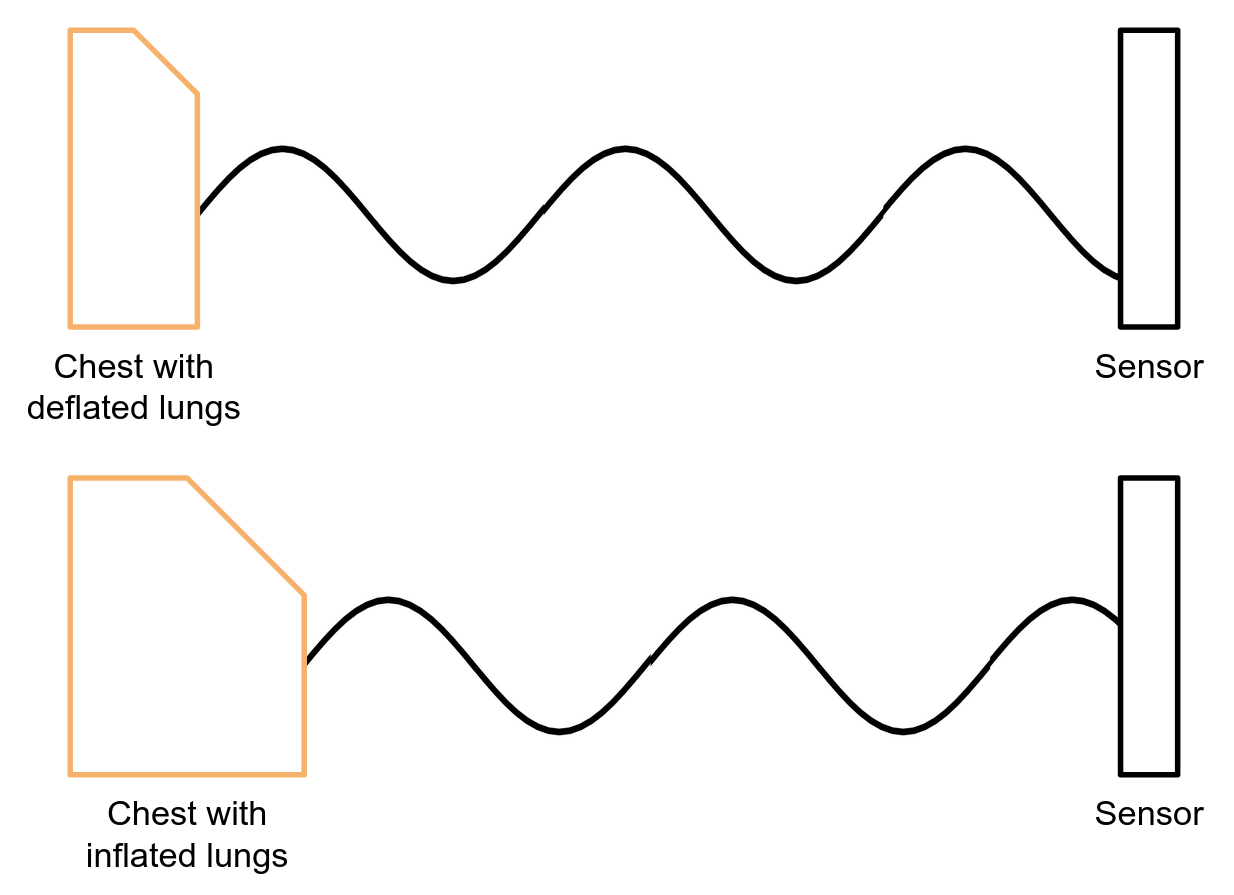
\includegraphics[width=.7\textwidth]{figures/measuring_vital_signs/phase_difference.png}
\caption{Exaggerated scheme on how the phase of the signal changes depending on the inflated or deflated chest of a person.}
\label{fig:phase_difference}
\end{figure}

\subsection{Phase unwrapping}
% - formula with the tan
% - unwrapping because of 2 pi
% - calculating the doppler?
Most existing solutions, like~\cite{li2009radar, yang2016monitoring, alizadeh2019remote} make use of phase extraction like in Figure~\ref{fig:phase_unwrapping}. From the radar data the range-FFT is calculated, on this FFT the peak is found. This peak denotes the location of the person. From that peak the phase is extracted and saved in a sliding window configuration. This same event repeats every 50 milliseconds. So, for each 50 milliseconds, the phase is extracted. All of these phase values form a waveform on their own, which can function as the input for the vital signs estimation. 

In the case of this project, the phase must be extracted from the generated heatmap. However, this means that the radar data is put through two more FFTs other than the range-FFT, namely the doppler-FFT and the azimuth-FFT. There were some concerns that the phase information would be lost during the generation of those two other FFTs, but during testing, it became apparent that the vital signs waveform could also be extracted from the phase of one bin in the heatmap. Because this is possible, information from a 2 dimensional space can be taken and processed to extract the vital signs. This is the second very important step that needs to be taken to arrive at the multiple person vital signs tracking goal. The first step is to track the persons in the radar view. This second step is to extract and unwrap the separate phase waveforms for each person. The next step is to take these waveforms and extract the vital signs data out of this data.

\begin{figure}[t]
\centering
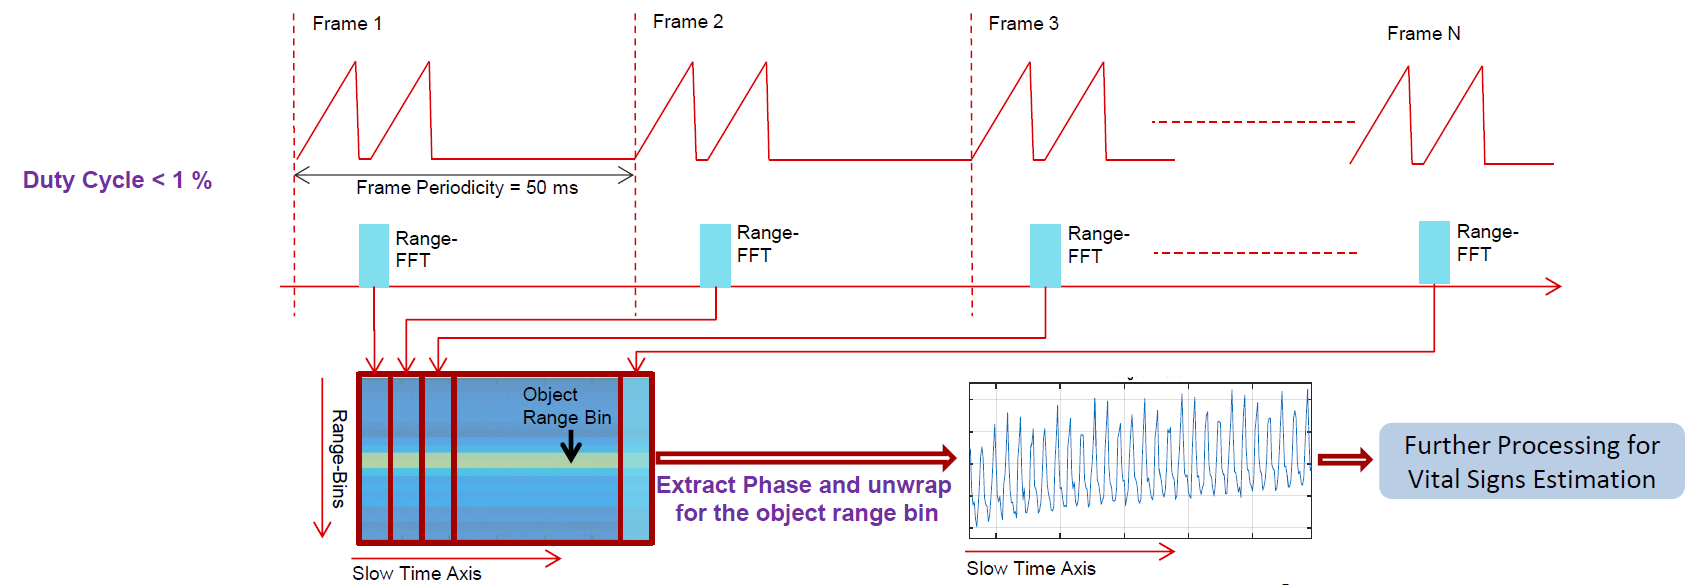
\includegraphics[width=.95\textwidth]{figures/measuring_vital_signs/phase_unwrapping.png}
\caption{Visual representation of how the phase gets unwrapped. Image has been taken from~\cite{vital_signs_lab_website}.}
\label{fig:phase_unwrapping}
\end{figure}

\section{Vital signs estimation}
% - difference is used between different phase values
% - Impulse noise filter
% - IIR biquad filter
% - breath circular buffer
% - heart circular buffer with motion detection
% - peak counting heart with filters
% - peak counting breath with filters
% - execute FFT on the breathing and heartrate estimation
% - peak counting and sorting again
Before starting with this section, I want to emphasize that I have copied these vital sign estimation implementations to a large extend from the TI Vital signs estimation demo~\cite{vital_signs_lab_website} and the Matlab implementation from my mentor Caitlin Ramsey~\cite{caitlin_msc_thesis_2020}. The main alterations I made was to make the code usable for multiple people at the same time. I chose for this approach because I am not very familiar with signal processing given my Embedded Systems background, so it is difficult to innovate in that field. Secondly, the main bulk of code is already implemented for this embedded platform, so it is a waste not to use it. I think it is important to explain the inner workings of this vital signs estimation implementation in this thesis, because it has a great significance to the project.

% TODO explain the contents of this section

\subsection{Data preparation}
The phase values coming from the heatmap are stored in circular buffers for further processing. But first, the data needs to be prepared. The algorithms work by using the phase changes. A phase change is computed by comparing the current phase by the previous phase value, like this:

\begin{equation}
    \label{eq:phase_difference}
    P_{old} = P_{current} - P_{previous}
\end{equation}

This results in an array with phase changes which can be used in processing. But first, the signal is cleaned up by an impulse noise filter. The data which is coming from the sensor is raw data. There can be unwanted spikes in the data, for example due to electromagnetic interference. This noise needs to be filtered out beforehand. This is done in a sliding window configuration, where the the three most recent values are stored. If the ratio between the first and the second, and the ratio between the third and the second are above a certain threshold, the second value will become an interpolation from the first and third value. This filter makes sure that there are no sudden peaks in the data, but that the signal is still able to change shape. Now that the signal is cleaned up, the next step is to differentiate between the heartrate and the breathing rate.

\subsection{Splitting the heartrate and breathing rate signal}
To do separate analysis on the breathing rate and the heartrate, the source signal needs to be separated into two. The way this is done, is by using an IIR filter.

IIR filters are one of two common digital signal processing (DSP) filter types~\cite{iir_info_website}. IIR stands for Infinite Impulse Response. The other common type is the Finite Impulse Response filter. These types of filters modify the frequency content of a signal. FIR filters and IIR filters are both part of the Linear Time Invariant (LTI) filter group. LTI filters can modify the phase and the amplitude of certain frequencies of a signal. These filters are most commonly used to remove undesired frequencies from an input signal. For example: the antenna of a car receives all of the radio stations at once, from 88 MHz to 108 MHz. To make it possible to only listen to a station at for example 89.9 MHz, a filter can be used to only allow the signal with a frequency of 89.9 MHz. The main difference between FIR and IIR sensors, is that the IIR sensors make use of a feedback mechanism. If the IIR filter is first zero and receives a 1 as an input, the filter output can (theoretically) never reach zero again. A FIR filter works with a certain amount of stages, and is able to reach zero after a certain amount of time. For this project an IIR filter is chosen because it is more efficient to implement for embedded devices, since it uses less memory and calculations compared to a similar FIR algorithm~\cite{iir_faq_website}. 

The IIR filter used in this project is an biquad cascade IIR algorithm. Biquad stands for biquadratic, which refers to the Z-domain, where the transfer function is a ratio of two quadratic functions:

\begin{equation}
\label{eq:biquad_filter_z}
    H(z)={\frac {b_{0}+b_{1}z^{-1}+b_{2}z^{-2}}{1+a_{1}z^{-1}+a_{2}z^{-2}}}
\end{equation}

The filter used in this project can be written down as an equation:

\begin{equation}
\label{eq:biquad_filter}
    y[n]=b_{0}x[n]+b_{1}x[n-1]+b_{2}x[n-2]-a_{1}y[n-1]-a_{2}y[n-2]
\end{equation}

\begin{figure}[t]
\centering
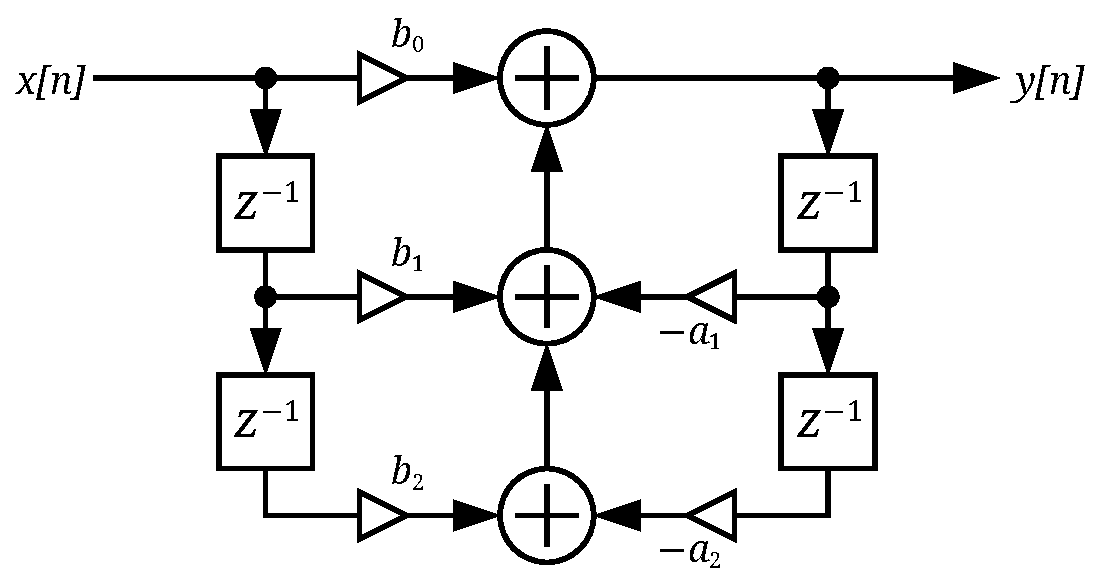
\includegraphics[width=.95\textwidth]{figures/measuring_vital_signs/Biquad_filter_DF-I.pdf}
\caption{The flow graph for a biquad cascade IIR filter. A more visual representation from Eq.~\ref{eq:biquad_filter}, how the input gets transformed to the output.}
\label{fig:iir_visual}
\end{figure}

A more visual flow graph can be found in Figure~\ref{fig:iir_visual}. This algorithm is translated in C code. This filter is executed on the input signal two times, once for the breathing rate waveform and once for the heartrate waveform. The filter is therefore configured like a bandpass filter. It will remove frequencies which are not in the allowed frequency range. The frequency ranges that were used in this project can be found in Table~\ref{tab:freq_ranges}.

\begin{table}[ht]
\centering
\begin{tabular}{|r|c|c|}
\hline
\textbf{Parameter} & \begin{tabular}[c]{@{}l@{}}\textbf{Minimum\\ frequency}\end{tabular} & \begin{tabular}[c]{@{}l@{}}Maximum \\ frequency\end{tabular} \\ \hline
Breathing rate & 0.1 Hz & 0.5 Hz \\
Heart rate & 0.8 Hz & 2.0 Hz \\ \hline
\end{tabular}
\caption{Typical frequency ranges from the breathing rate and heartrate. These frequency ranges are used in this project to filter out the right waveforms to do analysis on.}
\label{tab:freq_ranges}
\end{table}

So, there was one input signal, which is now split into two different signals, one for heart and one for breathing. The next step is to concentrate on getting a beats per minute (BPM) reading out of this data.

\subsection{Circular buffers}
The data from these two separate waveforms are stored in a circular buffer. The length of these buffers can be found in the configuration file in Table~\ref{tab:vs-parameter-config}.

\begin{table}[ht]
\centering
\begin{tabular}{|r|c|l|}
\hline
\textbf{Parameters} & \textbf{Values} & \textbf{Comments} \\ \hline
Start range (meters) & 0.1 & \begin{tabular}[c]{@{}l@{}}The persons to be detected \\ are expected to be within \\ the start range and the end \\ range from the sensor.\end{tabular} \\ \cline{1-2}
End range (meters) & 0.7 &  \\ \hline
Breathing waveform size & 256 & \begin{tabular}[c]{@{}l@{}}Specifies the number of points \\ within the waveforms. The \\ more data points are in the \\ circular buffer, the more data \\ is captured and the more \\ accurate the reading becomes. \\ A downside of using a large \\ waveform size is that it looses \\ the ability to capture \\ instantaneous changes.\end{tabular} \\ \cline{1-2}
Heartrate waveform size & 320 &  \\ \hline
Rx-antenna to process & 4 & \begin{tabular}[c]{@{}l@{}}Because there are 4 Rx antenna, \\ this value could be max. 4. \\ Because for this implementation \\ the rangeAzimuth-FFT is used, \\ only a value of 4 is allowed.\end{tabular} \\ \hline
\begin{tabular}[c]{@{}r@{}}Alpha filter value for \\ Breathing waveform\\ energy computation\end{tabular} & 0.1 & \begin{tabular}[c]{@{}l@{}}Alpha filter values for recursive \\ averaging of the waveform \\ energies based on the equation \\ below where x(n) is the current \\ waveform value while E(n) is the \\ energy. \\ E(n)=ax\textasciicircum{}2(n)+(1-a)E(n-1)\end{tabular} \\ \cline{1-2}
\begin{tabular}[c]{@{}r@{}}Alpha filter value for \\ heartrate waveform\\ energy computation\end{tabular} & 0.05 &  \\ \hline
\begin{tabular}[c]{@{}r@{}}Scale factor for the \\ breathing waveform\end{tabular} & 300000 & \begin{tabular}[c]{@{}l@{}}Scaling factors to convert \\ waveform values in floating \\ points to 32-bit integers \\ required for the FFT.\end{tabular} \\ \cline{1-2}
\begin{tabular}[c]{@{}r@{}}Scale factor for the \\ heartrate waveform\end{tabular} & 300000 &  \\ \hline
\end{tabular}
\caption{Overview of all of the Vital Signs configuration parameters getting send to the chip. These parameters mostly control the sensitivity of the chip. For each parameter, the value used in this project is mentioned and a short explanation. }
\label{tab:vs-parameter-config}
\end{table}